\documentclass[12pt]{article}

\usepackage{sbc-template}

\usepackage{graphicx,url}
\usepackage{float}
\usepackage[brazil]{babel}   
%\usepackage[latin1]{inputenc}  
\usepackage[utf8]{inputenc}  
% UTF-8 encoding is recommended by ShareLaTex
\usepackage{xcolor}
% Definindo novas cores
\definecolor{verde}{rgb}{0.25,0.5,0.35}
\definecolor{jpurple}{rgb}{0.5,0,0.35}
% Configurando layout para mostrar codigos Java
\usepackage{listings}
\lstset{
	language=Java,
	basicstyle=\ttfamily\small, 
	keywordstyle=\color{jpurple}\bfseries,
	stringstyle=\color{red},
	commentstyle=\color{verde},
	morecomment=[s][\color{blue}]{/**}{*/},
	extendedchars=true, 
	showspaces=false, 
	showstringspaces=false, 
	numbers=left,
	numberstyle=\tiny,
	breaklines=true, 
	backgroundcolor=\color{cyan!10}, 
	breakautoindent=true, 
	captionpos=b,
	xleftmargin=0pt,
	tabsize=4
}
\pagestyle{empty}
     
\sloppy

\title{Sistema Cliente Gerenciador de FTP \\ Exercício Computacional I}

\author{Rafael Gonçalves de Oliveria Vianal\inst{1} }


\address{Sistemas de Informação -- Universidade Federal do Mato Grosso do Sul
	(UFMS)\\
  	Caixa Postal 79400-000 -- Coxim -- MS -- Brazil
  \email{rafael.viana@aluno.ufms.br}
}

\begin{document} 

\maketitle

     
\begin{resumo} 
  Este relatório descreve como foi implementado um sistema cliente gerenciador de FTP, utilizando JavaFX como \textit{Graphical User Interface} e o Apache Commons Net 3.6, como biblioteca de conexão FTP.
\end{resumo}


\section{JavaFX}
Foi escolhido o JavaFX para criar uma interface gráfica onde o usuário terá um melhor desempenho, ao utilizar o sistema.
Para criar um sistema elegante foi utilizado uma biblioteca com novos elementos CSS, a bibliteca utilizada para essa finalidade foi  a \textbf{JFoenix}, essa bibliteca é opensorce e pode ser baixada no github https://github.com/jfoenixadmin/JFoenix, juntamente de seu documentação.
Para icones foi utilizado a biblioteca fontawesomefx-8.9 
	
\section{Apache Commons Net 3.6} \label{sec:firstpage}

Para melhor desempenho nas conexões ftp, foi utilizada a biblioteca de conexão FTP da Apache Commons, onde a mesma se encontra na versão 3.6 current.

\section{Problematica}
O trabalho proposto tem como objetivo criar um Cliente FTP, onde Adicione, Edite, Baixe e faz Upload de arquivos e pastas, porem apenas 5 pastas e 2 arquivos por diretorio sendo que no máximo deve ter 3 níveis.
Um problema identificado e referênte a segurança desses pré-requisitos, onde que em um Cliente FTP a segurança da validação desses requisitos e inteiramente do Software Cliente é não do servidor, sendo assim para interece academico as validações devem ser inteiramente do SERVIDOR FTP não do CLIENTE FTP.

\section{References}

Bibliographic references must be unambiguous and uniform.  We recommend giving
the author names references in brackets, e.g. \cite{knuth:84},
\cite{boulic:91}, and \cite{smith:99}.

The references must be listed using 12 point font size, with 6 points of space
before each reference. The first line of each reference should not be
indented, while the subsequent should be indented by 0.5 cm.

\bibliographystyle{sbc}
\bibliography{sbc-template}

\section{Anexos}
A estrutura do código foi dividida em 3 pastas sendo elas Cliente, Icons e Socket.

\begin{enumerate}
	
\item{A pasta cliente é responsável pela parte de Interface Gráfica do Usuário, envolvendo controllers.}
\item{A pasta Icons armazena icons utilizados na pasta cliente.}
\item{A pasta socket e responsável por toda comunicação da Lib da Apache com os controllers do cliente.}

\end{enumerate}

	


\begin{figure}[H]
	\centering
	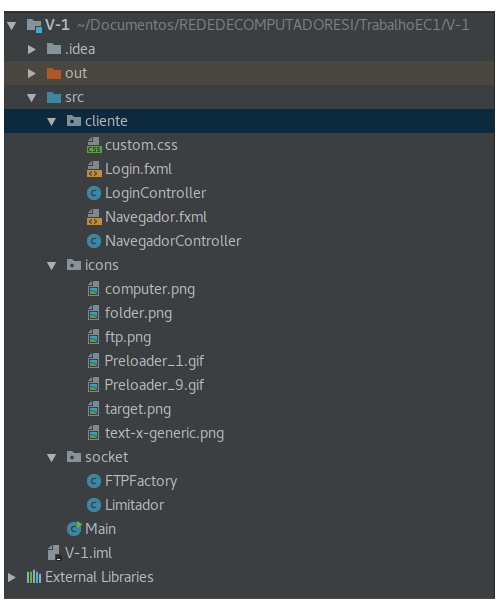
\includegraphics[width=.3\textwidth]{Imagens/001.png}
	\caption{ Imagem da Tela de Login.}
	\label{fig:01}
\end{figure}


Primeiramente a Class Main e invocada, chamando a Scene do Login.fxml, o controller do login e responsável por fornecer o necessario para o FTPClient poder fazer a conexão.

\begin{lstlisting}

public class Main  extends Application{

@Override
	public void start(Stage stage) throws Exception {
	Parent root = FXMLLoader.load(getClasssingleton().getResource("/cliente/Login.fxml"));
	Scene scene = new Scene(root);
	stage.setScene(scene);
	stage.show();
}


public static void main(String[] args) {
	launch(args);

}

}

\end{lstlisting}

\begin{figure}[H]
	\centering
	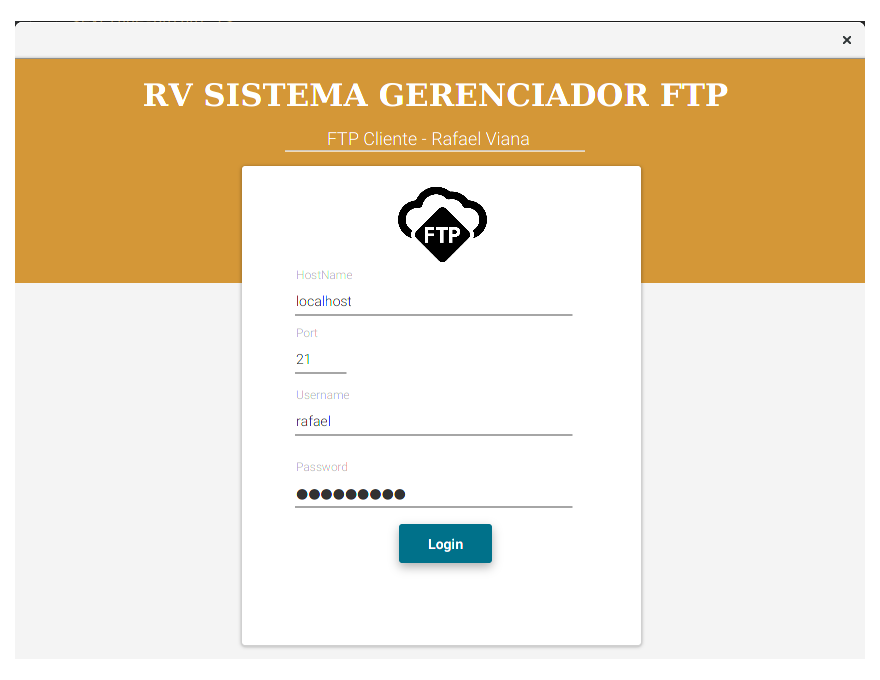
\includegraphics[width=.9\textwidth]{Imagens/01.png}
	\caption{ Imagem da Tela de Login.}
	\label{fig:01}
\end{figure}

Com a tela de login aberta o usuário entra com as informações login , senha, endereço do host, port do host mostrado no código abaixo.
\vspace{.4cm}
\begin{lstlisting}
private void login(ActionEvent event) {
	btnLogin.setVisible(false);
	imgProgress.setVisible(true);
	
	PauseTransition pauseTransition = new PauseTransition();
	pauseTransition.setDuration(Duration.seconds(3));
	pauseTransition.setOnFinished(ev -> {

try {
	
	int reply = FTPFactory.getInstance().FTPConecta(txtHostName.getText(),Integer.parseInt(txtHostPort.getText()),this.txtUsername.getText(),this.txtPassword.getText());
	System.out.println("Igual:" + reply);
	
	if (reply == 230) {
	
		btnLogin.getScene().getWindow().hide();
		completeLogin();
	
	} else {
	
		imgProgress.setVisible(false);
		btnLogin.setVisible(true);
		JOptionPane.showMessageDialog(null,"Erro Senha ou Usuário incorreto !!", "Erro ao Logar",JOptionPane.ERROR_MESSAGE);
	}

} catch (IOException ex) {
	Logger.getLogger(LoginController.class.getName()).log(Level.SEVERE, null, ex);
} catch (Exception ex) {
	Logger.getLogger(LoginController.class.getName()).log(Level.SEVERE, null, ex);
}

});
  pauseTransition.play();
}

private void completeLogin() throws IOException {
	
	imgProgress.setVisible(false);
	Stage dashboardStage = new Stage();
	dashboardStage.setTitle("");
	Parent root = FXMLLoader.load(getClass().getResource("Navegador.fxml"));
	Scene scene = new Scene(root);
	dashboardStage.setScene(scene);
	dashboardStage.show();
	
}

\end{lstlisting}


Para poder realizar a comunicação entre as classes e o FTPClient da apache, foi criado uma classe singleton chamada de FTPFactory onde a mesma cria uma getInstance de FTPClient, podendo ser chamada de qualquer classe sem ter que que ser instanciada novamente, oque iria ocasionar a perda da conexão FTP.

\begin{lstlisting}

public class FTPFactory {
	
	private final FTPClient ftp;
	private TreeItem<FTPFile> file;
		
	private FTPFactory() {
			this.ftp = new FTPClient();
	}
	
	public static FTPFactory getInstance() {
	
		return FTPFactoryHolder.INSTANCE;
	}


	/**
	* Classe privada que armazena a única instância de FTPFactory.
	*/
	private static class FTPFactoryHolder {
	
		private static final FTPFactory INSTANCE = new FTPFactory();
	}


	public FTPClient getFTP() {
		return this.ftp;
	}


	public boolean Excluir(FTPFile file) {
	try {
			if (file.isDirectory()) {
				System.out.println(file.getLink());
				return ftp.removeDirectory(file.getLink());
			} else {
				System.out.println(file.getLink());
				return ftp.deleteFile(file.getLink());
			}
	} catch (IOException e) {
		e.printStackTrace();
		}	
		return false;
	}


	public int FTPConecta(String host, int port, String user, String pwd) throws Exception {
		int reply;
		ftp.connect(host, port);
		reply = ftp.getReplyCode();
		if (!FTPReply.isPositiveCompletion(reply)) {
			ftp.disconnect();
			throw new Exception("Exception in connecting to FTP Server");
		}
		ftp.login(user, pwd);
		reply = ftp.getReplyCode();
		ftp.setFileType(FTPClient.BINARY_FILE_TYPE);
		ftp.enterLocalPassiveMode();
		ftp.setAutodetectUTF8(true);
		return reply;
	}


	public void disconnect() {
		if (this.ftp.isConnected()) {
		try {
			this.ftp.logout();
			this.ftp.disconnect();
			} catch (IOException f) {
	
			}
	    }
	}
}	

\end{lstlisting}

Após a Class login em conjunto com a Class FTPFactor, validar os dados de usuário a tela de navegação e aberta, essa tela nada mais é do que um conjunto de botões em uma Grid a esquerda e um TreeView do JavaFX no centro para poder navegar pela estutura dos diretórios.

\begin{figure}[H]
	\centering
	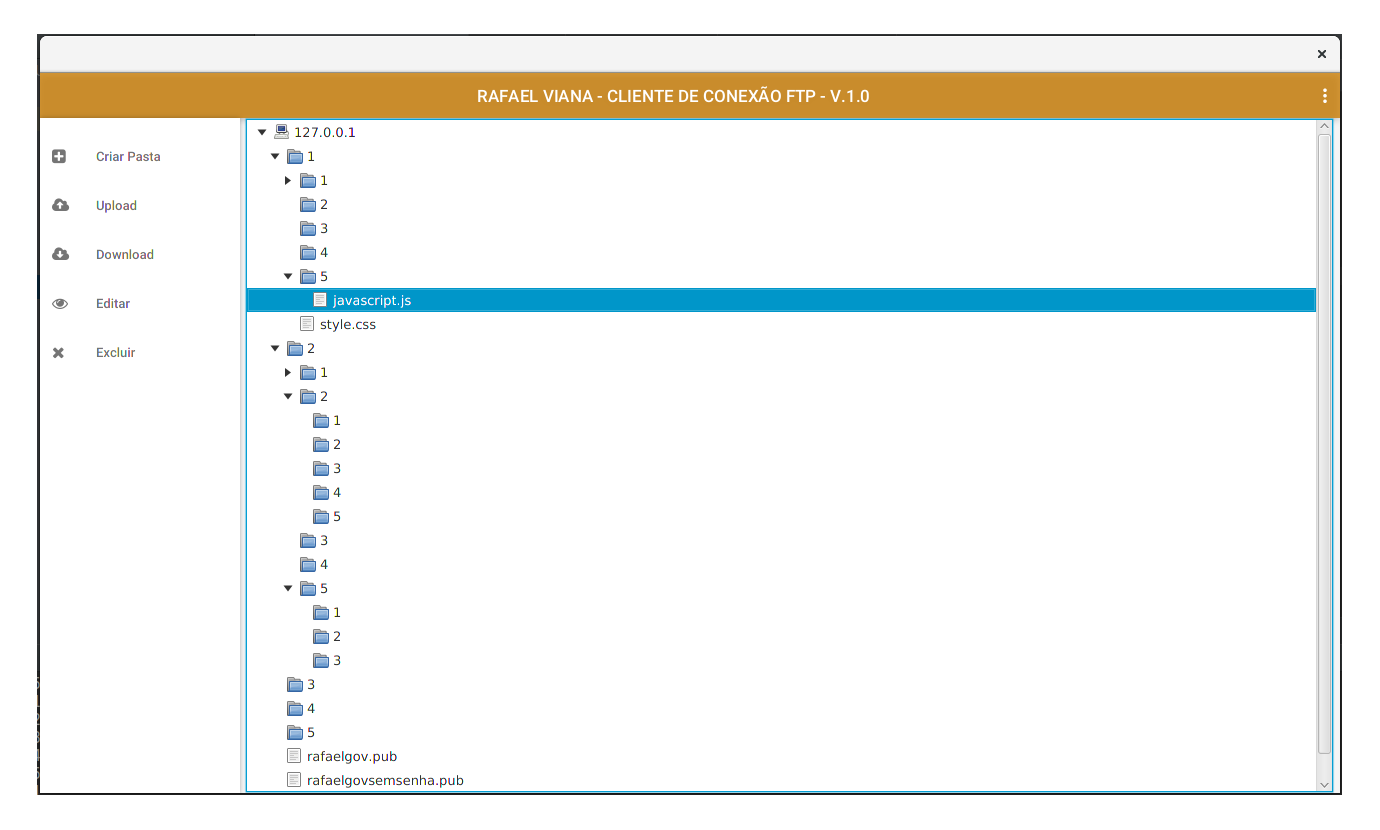
\includegraphics[width=0.8\textwidth]{Imagens/02.png}
	\caption{ Imagem da Tela de Navegação.}
	\label{fig:01}
\end{figure}


Toda lógica de abastecimento da TreeView e criação dos ItemView utilizados na TreeView estão no código de criação da tela de navegação,o método Navegação inicia a criação dos ItemViws e toda a estrutura da arvore como ADICIONAR, REMOVER, LISTAR, EDITAR, BAIXAR e UPLOAD de arquivos/pastas, o método getNodesForDirectory() cria recursivamente Nodes/ItemView encadeando seus filhos na TreeView, facilitando assim a navegação.

\begin{lstlisting}
 private void Navegacao() throws IOException {
	FTPFile files[];
	
	
	TreeItem<FTPFile> treeRoot;
	
	files = FTPFactory.getInstance().getFTP().listFiles();
	Tree.setEditable(true);
	
	if (files != null && files.length > 0) {
		files[0].setRawListing(FTPFactory.getInstance().getFTP().getPassiveHost());
		treeRoot = getNodesForDirectory(files[0], true);
	} else {
		FTPFile file = new FTPFile();
		file.setType(FTPFile.DIRECTORY_TYPE);
		file.setLink(FTPFactory.getInstance().getFTP().printWorkingDirectory());
		file.setRawListing(FTPFactory.getInstance().getFTP().getPassiveHost());
		treeRoot = new TreeItem<>(file, new ImageView(computador));
	}
	Tree.getSelectionModel().select(treeRoot);
	Tree.setRoot(treeRoot);
	
	
	btnBaixar.disableProperty().bind(Tree.getSelectionModel().selectedItemProperty().isNull()
	.or(Tree.getSelectionModel().selectedItemProperty().isEqualTo(treeRoot)));
	
	
	btnBaixar.setOnAction(e -> {
		TreeItem<FTPFile> selected = Tree.getSelectionModel().getSelectedItem();
		if (selected.getValue().isFile()) {
			JFileChooser local = new JFileChooser();
			local.setFileSelectionMode(JFileChooser.DIRECTORIES_ONLY);
			local.setDialogTitle("Escolha um local para salvar");
			local.setFileHidingEnabled(false);
			int res = local.showSaveDialog(null);
			if (res == JFileChooser.APPROVE_OPTION) {
				String caminho = String.valueOf(local.getSelectedFile());
				try {
					FileOutputStream fos = new FileOutputStream(caminho);
					if (FTPFactory.getInstance().getFTP().retrieveFile(selected.getValue().getLink(), fos)) {
						JOptionPane.showMessageDialog(null, "Arquivo Baixado com Sucesso!" + "\n\n",
						"Sucesso", JOptionPane.INFORMATION_MESSAGE);
					}
					
				} catch (FileNotFoundException e1) {
					e1.printStackTrace();
				} catch (Exception ex) {
					JOptionPane.showMessageDialog(null, "Erro ao Baixado  Arquivo : " + ex.getMessage(), "Erro", JOptionPane.ERROR_MESSAGE);
				}
			}
		} else {
			JOptionPane.showMessageDialog(null, "Somente Arquivos!" + "\n\n",
			"Erro", JOptionPane.ERROR_MESSAGE);
		}
	});
	
	
	btnUp.setOnAction(e -> {
		TreeItem<FTPFile> selected = Tree.getSelectionModel().getSelectedItem();
		try {
			FTPFactory.getInstance().getFTP().changeWorkingDirectory(selected.getValue().getLink());
			if (limiteNivel() <= 5) {
				if (limiteArquivo()) {
					JFileChooser fc = new JFileChooser();
					fc.setFileSelectionMode(JFileChooser.FILES_ONLY);
					int result = fc.showOpenDialog(null);
					if (result == JFileChooser.APPROVE_OPTION) {
						File arquivo = fc.getSelectedFile();
						InputStream isArquivo = null;
						try {
							isArquivo = new FileInputStream(arquivo.getAbsolutePath());
						} catch (FileNotFoundException e1) {
							e1.printStackTrace();
						}
						try {
							FTPFile f = new FTPFile();
							
							if (selected.getValue().isDirectory()) {
								FTPFactory.getInstance().getFTP().changeWorkingDirectory(selected.getValue().getLink());
								f.setLink(selected.getValue().getLink() + separador + arquivo.getName());
							} else {
								FTPFactory.getInstance().getFTP().changeWorkingDirectory(selected.getParent().getValue().getLink());
								f.setLink(selected.getParent().getValue().getLink() + separador + arquivo.getName());
							}
							
							if (FTPFactory.getInstance().getFTP().storeFile(arquivo.getName(), isArquivo)) {
								
								f.setName(arquivo.getName());
								f.setRawListing(arquivo.getName());
								f.setType(FTPFile.FILE_TYPE);
								TreeItem<FTPFile> newItem = new TreeItem<FTPFile>(f, new ImageView(this.arquivo));
								if (selected.getValue().isDirectory()) {
									selected.getChildren().add(newItem);
								} else {
									selected.getParent().getChildren().add(newItem);
								}
								
								JOptionPane.showMessageDialog(null, "Arquivo Enviado!");
							} else {
								JOptionPane.showMessageDialog(null, "Arquivo não enviado!");
							}
							
							
						} catch (IOException e1) {
							e1.printStackTrace();
						}
						
					} else {
						JOptionPane.showMessageDialog(null, "Arquivo não selecionado!");
					}
				} else {
					JOptionPane.showMessageDialog(null, "Apenas 2 arquivos por pasta", "Limite Atingido", JOptionPane.WARNING_MESSAGE);
				}
			} else {
				JOptionPane.showMessageDialog(null, "Apenas 3 níveis de Diretórios", "Limite Atingido", JOptionPane.WARNING_MESSAGE);
				
			}
		} catch (IOException e1) {
			e1.printStackTrace();
		}
	});
	
	
	btnEditar.setOnAction(e -> {
		TreeItem<FTPFile> selected = Tree.getSelectionModel().getSelectedItem();
		String novolink = "";
		if (selected.getParent().getValue() != null) {
			
			try {
				FTPFactory.getInstance().getFTP().changeWorkingDirectory(selected.getParent().getValue().getLink());
				novolink = FTPFactory.getInstance().getFTP().printWorkingDirectory();
			} catch (IOException e1) {
				e1.printStackTrace();
			}
			try {
				String novoNome = JOptionPane.showInputDialog("Digite um novo nome para " + selected.getValue().getName());
				
				if (FTPFactory.getInstance().getFTP().rename(selected.getValue().getName(), novoNome)) {
					selected.getValue().setRawListing(novoNome);
					selected.getValue().setLink(novolink + separador + novoNome);
					Tree.refresh();
				}
			} catch (IOException e1) {
				e1.printStackTrace();
			}
		}
		
	});
	
	btnEditar.disableProperty().bind(Tree.getSelectionModel().selectedItemProperty().isNull()
	.or(Tree.getSelectionModel().selectedItemProperty().isEqualTo(treeRoot)));
	
	
	btnExcluir.setOnAction(e -> {
		TreeItem<FTPFile> selected = Tree.getSelectionModel().getSelectedItem();
		int reply = JOptionPane.showConfirmDialog(null, "Deseja deletar esse arquivo ?", "Confirma Exclusão", JOptionPane.YES_NO_OPTION);
		if (reply == JOptionPane.YES_OPTION) {
			if (FTPFactory.getInstance().Excluir(selected.getValue())) {
				System.out.println(selected.getValue().getLink());
				selected.getParent().getChildren().remove(selected);
				JOptionPane.showMessageDialog(null, "Excluido ", "OK", JOptionPane.INFORMATION_MESSAGE);
			} else {
				JOptionPane.showMessageDialog(null, "Erro ao excluir arquivo ", "Erro", JOptionPane.WARNING_MESSAGE);
			}
		}
		
	});
	
	
	btnExcluir.disableProperty().bind(Tree.getSelectionModel().selectedItemProperty().isNull()
	.or(Tree.getSelectionModel().selectedItemProperty().isEqualTo(treeRoot)));
	
	TextField textField = new TextField();
	
	
	EventHandler<ActionEvent> addAction = e -> {
		try {
			TreeItem<FTPFile> selected = Tree.getSelectionModel().getSelectedItem();
			FTPFactory.getInstance().getFTP().changeWorkingDirectory(selected.getValue().getLink());
			if (limiteNivel() <= 5) {
				if (limitePasta()) {
					if (selected == null) {
						selected = treeRoot;
					}
					String text = JOptionPane.showInputDialog("Nome da Pasta");
					if (text.isEmpty()) {
						text = "NovaPasta";
					}
					FTPFile f = new FTPFile();
					f.setType(FTPFile.DIRECTORY_TYPE);
					f.setRawListing(text);
					f.setName(text);
					TreeItem<FTPFile> newItem = new TreeItem<FTPFile>(f, new ImageView(pasta));
					
					if (selected.getValue().isDirectory()) {
						f.setLink(selected.getValue().getLink() +separador + text);
						System.out.println("Link: " + f.getLink());
						if (FTPFactory.getInstance().getFTP().makeDirectory(f.getLink())) {
							selected.getChildren().add(newItem);
							Tree.getSelectionModel().select(newItem);
						} else {
							JOptionPane.showMessageDialog(null, "Erro pasta nao pode ser criado com esse nome.", "Diretório Existente", JOptionPane.WARNING_MESSAGE);
						}
					} else {
						if (selected.getParent().getValue() != null) {
							f.setLink(selected.getParent().getValue().getLink() + separador + text);
							System.out.println("Link: " + f.getLink());
							if (FTPFactory.getInstance().getFTP().makeDirectory(f.getLink())) {
								selected.getParent().getChildren().add(newItem);
								Tree.getSelectionModel().select(newItem);
							} else {
								JOptionPane.showMessageDialog(null, "Erro pasta nao pode ser criado com esse nome.", "Diretório Existente", JOptionPane.WARNING_MESSAGE);
							}
						}
						
					}
					
				} else {
					JOptionPane.showMessageDialog(null, "Apenas 5 pastas por Diretório", "Limite Atingido", JOptionPane.WARNING_MESSAGE);
					
				}
			} else {
				JOptionPane.showMessageDialog(null, "Apenas 3 níveis de Diretórios", "Limite Atingido", JOptionPane.WARNING_MESSAGE);
				
			}
		} catch (IOException e1) {
			e1.printStackTrace();
		}
	};
	textField.setOnAction(addAction);
	btnAdd.setOnAction(addAction);
	
}


public TreeItem<FTPFile> getNodesForDirectory(FTPFile directory, boolean v) throws IOException {
	TreeItem<FTPFile> root;
	if (v) {
		directory.setType(FTPFile.DIRECTORY_TYPE);
		directory.setLink(FTPFactory.getInstance().getFTP().printWorkingDirectory());
		root = new TreeItem<FTPFile>(directory, new ImageView(computador));
		
	} else {
		root = new TreeItem<FTPFile>(directory, new ImageView(pasta));
	}
	FTPFile[] files = FTPFactory.getInstance().getFTP().listFiles();
	for (FTPFile f : files) {
		System.out.println("Carregando .. " + f.getName());
		if (f.isDirectory()) {
			FTPFactory.getInstance().getFTP().changeWorkingDirectory(f.getName());
			f.setLink(FTPFactory.getInstance().getFTP().printWorkingDirectory());
			System.out.println(f.getLink());
			root.getChildren().add(getNodesForDirectory(f, false));
		} else {
			f.setLink(FTPFactory.getInstance().getFTP().printWorkingDirectory() + separador + f.getName());
			root.getChildren().add(new TreeItem<FTPFile>(f, new ImageView(this.arquivo)));
		}
	}
	FTPFactory.getInstance().getFTP().changeToParentDirectory();
	return root;
}

\end{lstlisting}

Um dos objetivos do trabalho era limitar o cliente FTP, fazendo com que usuários que utilizarem o sistema só poderam criar 5 pastas e 2 arquivos por diretório, sendo que poderá no máximo ter 3 níveis de diretórios.
A classe Limitador do pacote Socket e responsável por fazer a armazenagem da quantidade Máxima de Pastas e Arquivos. Sendo utilizada na classe Navegação do pacote Cliente.
 
 \begin{lstlisting}
public class Limitador {

	private int p;
	private int a;
	
	public Limitador(int p, int a) {
		this.p = p;
		this.a = a;
	}
	
	public int getMP() {
		return p;
	}
	
	public int getMA() {
		return a;
	}

}
 \end{lstlisting}

Na classe Navegação do pacote cliente 3 métodos fazem parte da lógica empregada na Class Limitador sendo las.

\begin{lstlisting}

private boolean limiteArquivo() throws IOException {
	int num = FTPFactory.getInstance().getFTP().listDirectories().length;
	int numa = FTPFactory.getInstance().getFTP().listFiles().length - num;
	return numa < limite.getMA();
}

private boolean limitePasta() throws IOException {
	int num_diretorios = FTPFactory.getInstance().getFTP().listDirectories().length;
	return num_diretorios < limite.getMP();
}

private int limiteNivel() throws IOException {
	int num = FTPFactory.getInstance().getFTP().printWorkingDirectory().split("separador").length;
	return num;
}
\end{lstlisting}
\end{document}


